\documentclass[aspectratio=169,11pt]{beamer}
\usetheme[progressbar=frametitle, numbering=fraction]{metropolis}
% Preambul comun (documentație + prezentare folosesc aceleași figuri).
\usepackage{fontspec}
\usepackage[romanian]{babel}
\usepackage{csquotes}
\usepackage{newunicodechar}
% Simboluri absente din Latin Modern: le compunem în modul matematic.
\newunicodechar{≈}{\ensuremath{\approx}}
\newunicodechar{≤}{\ensuremath{\leq}}
\newunicodechar{≥}{\ensuremath{\geq}}
\newunicodechar{↔}{\ensuremath{\leftrightarrow}}
\usepackage{amsmath,amssymb}
\usepackage{xcolor}
\usepackage{tikz}
\usetikzlibrary{arrows.meta,positioning,shapes.geometric,shapes.multipart,fit,backgrounds,calc,decorations.pathreplacing,matrix}
\usepackage{pgfplots}
\pgfplotsset{compat=1.18}
% Format numeric românesc pe axe: 60.000 și 0,8.
\pgfkeys{/pgf/number format/.cd, use comma, 1000 sep={.}}
\usepgfplotslibrary{groupplots}

% Paletă (accesibilă, distinctă în alb-negru prin marcaje).
\definecolor{c1}{HTML}{2F6FDE}
\definecolor{c2}{HTML}{E07B39}
\definecolor{c3}{HTML}{1F9D63}
\definecolor{c4}{HTML}{8E5CC4}
\definecolor{c5}{HTML}{C8423B}
\definecolor{c6}{HTML}{6B7280}
\definecolor{boxbg}{HTML}{F3F5F9}

\pgfplotscreateplotcyclelist{spd}{
  {c1,mark=*,thick},{c2,mark=square*,thick},{c3,mark=triangle*,thick},
  {c4,mark=diamond*,thick},{c5,mark=pentagon*,thick},{c6,mark=o,thick,dashed}}
\pgfplotsset{
  every axis/.append style={cycle list name=spd, grid=major, grid style={gray!25},
    tick label style={font=\footnotesize}, label style={font=\small},
    legend style={font=\footnotesize, draw=none, fill=white, fill opacity=0.85, text opacity=1},
    legend cell align=left},
}

% Axe de debit în mii: 60k în loc de 60.000.
\pgfplotsset{kticks/.style={scaled y ticks=base 10:-3, ytick scale label code/.code={},
  yticklabel={\pgfmathprintnumber[fixed,precision=0]{\tick}k}}}

\tikzset{
  comp/.style={draw, rounded corners=3pt, fill=boxbg, minimum height=8mm, minimum width=22mm, align=center, font=\small},
  store/.style={draw, cylinder, shape border rotate=90, aspect=0.25, fill=boxbg, minimum height=11mm, minimum width=18mm, align=center, font=\small},
  arr/.style={-{Stealth[length=2.2mm]}, thick},
  darr/.style={{Stealth[length=2.2mm]}-{Stealth[length=2.2mm]}, thick},
  note/.style={font=\scriptsize, text=black!65, align=center},
}

\usepackage{booktabs}
\newcommand{\datadir}{../docs/data/}
\InputIfFileExists{../docs/data/numbers.tex}{}{}
\providecommand{\R}[1]{??}
\setbeamercolor{progress bar}{fg=c1}
\setbeamercolor{frametitle}{bg=black!85}
\setbeamercolor{alerted text}{fg=c2}

\title{Memory cache pentru aplicații web}
\subtitle{Tabele in-memory + bază de date relațională — implementare distribuită în Rust și evaluarea performanțelor}
\author{Cristi Miloiu}
\institute{Proiect individual — aplicații paralele și distribuite}
\date{\today}

\begin{document}
\maketitle

\begin{frame}{Problema}
  \begin{columns}[T]
    \column{0.55\textwidth}
    \begin{itemize}
      \item Magazin online: \alert{100k produse}, 500k recenzii, 200 de categorii în PostgreSQL
      \item Trafic dominat de citiri (90–99\%), popularitate \alert{Zipf}
      \item Fiecare citire = join + agregare în DB
      \item Întrebarea: \emph{debit maxim, latență minimă, date corecte, memorie limitată, mai multe mașini?}
    \end{itemize}
    \column{0.42\textwidth}
    \[ T_{\text{mediu}} = T_{\text{cache}} + (1-h)\,T_{\text{DB}} \]
    \vspace{2mm}
    \small Rata de hit $h$ domină: de la 90\% la 99\% = de 10× mai puține interogări DB.
  \end{columns}
\end{frame}

\begin{frame}{Secvențial vs. paralel și distribuit}
  \centering\resizebox{0.85\linewidth}{!}{% Arhitectura secvențială vs paralelă/distribuită.
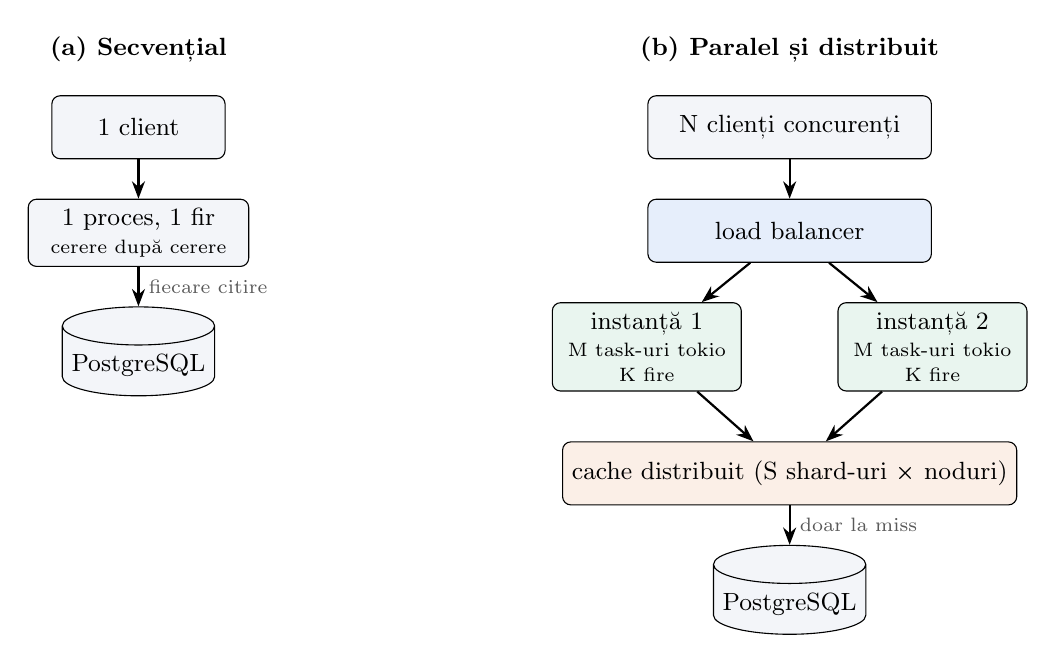
\begin{tikzpicture}[node distance=5mm and 7mm]
  \node[font=\small\bfseries] (t1) {(a) Secvențial};
  \node[comp, below=3mm of t1] (c1) {1 client};
  \node[comp, below=of c1, minimum width=28mm] (p1) {1 proces, 1 fir\\[-1pt]\scriptsize cerere după cerere};
  \node[store, below=of p1] (d1) {PostgreSQL};
  \draw[arr] (c1) -- (p1); \draw[arr] (p1) -- node[note, right] {fiecare citire} (d1);

  \node[font=\small\bfseries, right=50mm of t1] (t2) {(b) Paralel și distribuit};
  \node[comp, below=3mm of t2, minimum width=36mm] (c2) {N clienți concurenți};
  \node[comp, below=of c2, minimum width=36mm, fill=c1!12] (lb) {load balancer};
  \node[comp, below left=5mm and -12mm of lb, minimum width=24mm, fill=c3!10] (i1) {instanță 1\\[-1pt]\scriptsize M task-uri tokio\\[-2pt]\scriptsize K fire};
  \node[comp, below right=5mm and -12mm of lb, minimum width=24mm, fill=c3!10] (i2) {instanță 2\\[-1pt]\scriptsize M task-uri tokio\\[-2pt]\scriptsize K fire};
  \node[comp, below=12mm of $(i1)!0.5!(i2)$, minimum width=42mm, fill=c2!12] (cc) {cache distribuit (S shard-uri × noduri)};
  \node[store, below=of cc] (d2) {PostgreSQL};
  \draw[arr] (c2) -- (lb); \draw[arr] (lb) -- (i1); \draw[arr] (lb) -- (i2);
  \draw[arr] (i1) -- (cc); \draw[arr] (i2) -- (cc);
  \draw[arr] (cc) -- node[note, right] {doar la miss} (d2);
\end{tikzpicture}
}
\end{frame}

\begin{frame}{Arhitectura}
  \centering\resizebox{!}{0.82\textheight}{% Arhitectura distribuită (docker compose).
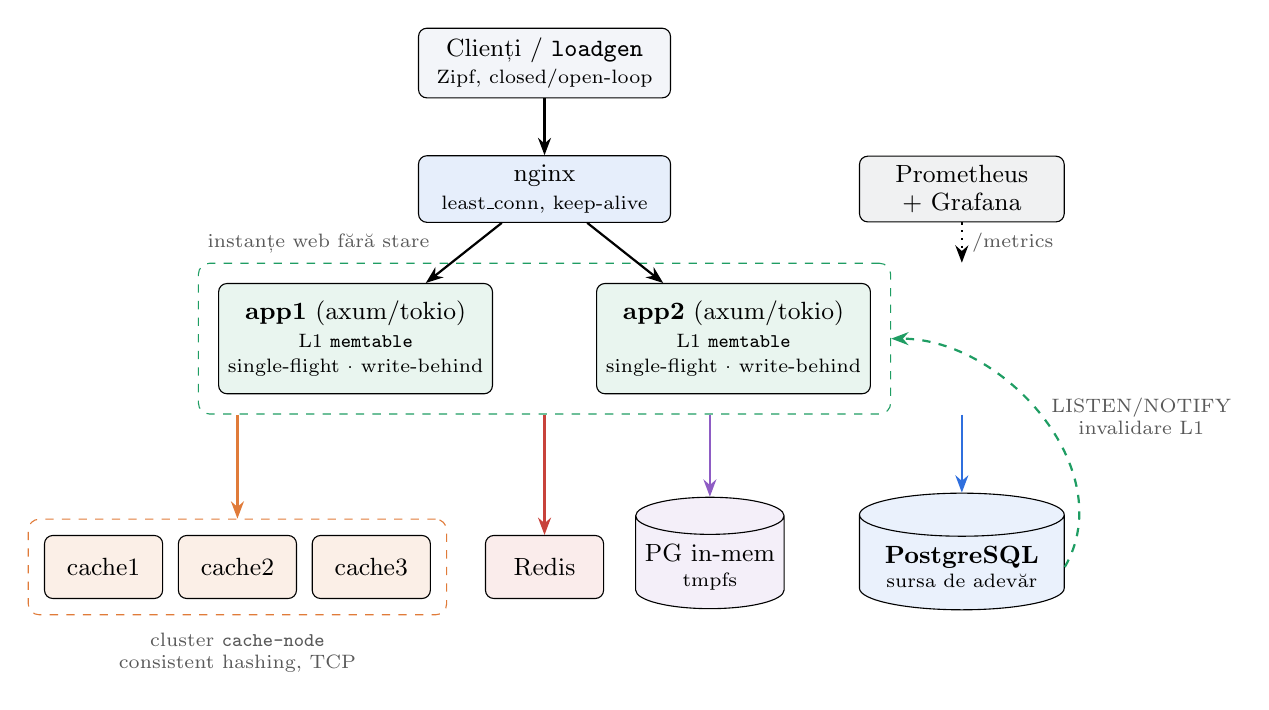
\begin{tikzpicture}
  \node[comp, minimum width=32mm] (cli) at (0,0) {Clienți / \texttt{loadgen}\\[-1pt]\scriptsize Zipf, closed/open-loop};
  \node[comp, minimum width=32mm, fill=c1!12] (lb) at (0,-1.6) {nginx\\[-1pt]\scriptsize least\_conn, keep-alive};
  \node[comp, minimum width=34mm, minimum height=14mm, fill=c3!10] (a1) at (-2.4,-3.5) {\textbf{app1} (axum/tokio)\\[-1pt]\scriptsize L1 \texttt{memtable}\\[-2pt]\scriptsize single-flight · write-behind};
  \node[comp, minimum width=34mm, minimum height=14mm, fill=c3!10] (a2) at (2.4,-3.5) {\textbf{app2} (axum/tokio)\\[-1pt]\scriptsize L1 \texttt{memtable}\\[-2pt]\scriptsize single-flight · write-behind};
  \begin{scope}[on background layer]
    \node[draw=c3, dashed, rounded corners, fit=(a1)(a2), inner sep=2.5mm] (apps) {};
  \end{scope}
  \node[note, anchor=south west] at (apps.north west) {instanțe web fără stare};
  \draw[arr] (cli) -- (lb);
  \draw[arr] (lb) -- (a1); \draw[arr] (lb) -- (a2);

  % Backend-uri.
  \node[comp, minimum width=15mm, fill=c2!12] (n1) at (-5.6,-6.4) {cache1};
  \node[comp, minimum width=15mm, fill=c2!12] (n2) at (-3.9,-6.4) {cache2};
  \node[comp, minimum width=15mm, fill=c2!12] (n3) at (-2.2,-6.4) {cache3};
  \begin{scope}[on background layer]
    \node[draw=c2, dashed, rounded corners, fit=(n1)(n3), inner sep=2mm] (ring) {};
  \end{scope}
  \node[note, below=1mm of ring] {cluster \texttt{cache-node}\\consistent hashing, TCP};
  \node[comp, minimum width=15mm, fill=c5!10] (rd) at (0,-6.4) {Redis};
  \node[store, fill=c4!10] (pm) at (2.1,-6.4) {PG in-mem\\[-2pt]\scriptsize tmpfs};
  \node[store, minimum width=26mm, minimum height=13mm, fill=c1!10] (db) at (5.3,-6.4) {\textbf{PostgreSQL}\\[-2pt]\scriptsize sursa de adevăr};

  \foreach \t/\c in {ring/c2, rd/c5, pm/c4, db/c1} {
    \draw[arr, \c] (apps.south -| \t.north) -- (\t.north);
  }
  \draw[arr, dashed, c3] (db.east) to[out=60,in=0] node[note, right, pos=0.5] {LISTEN/NOTIFY\\invalidare L1} (apps.east);

  \node[comp, minimum width=26mm, fill=c6!10] (obs) at (5.3,-1.6) {Prometheus\\[-1pt]+ Grafana};
  \draw[arr, dotted] (obs.south) -- node[note, right] {/metrics} (obs.south |- apps.north);
\end{tikzpicture}
}
\end{frame}

\begin{frame}{Motorul \texttt{memtable}}
  \centering\resizebox{0.8\linewidth}{!}{% Structura internă a unei tabele memtable.
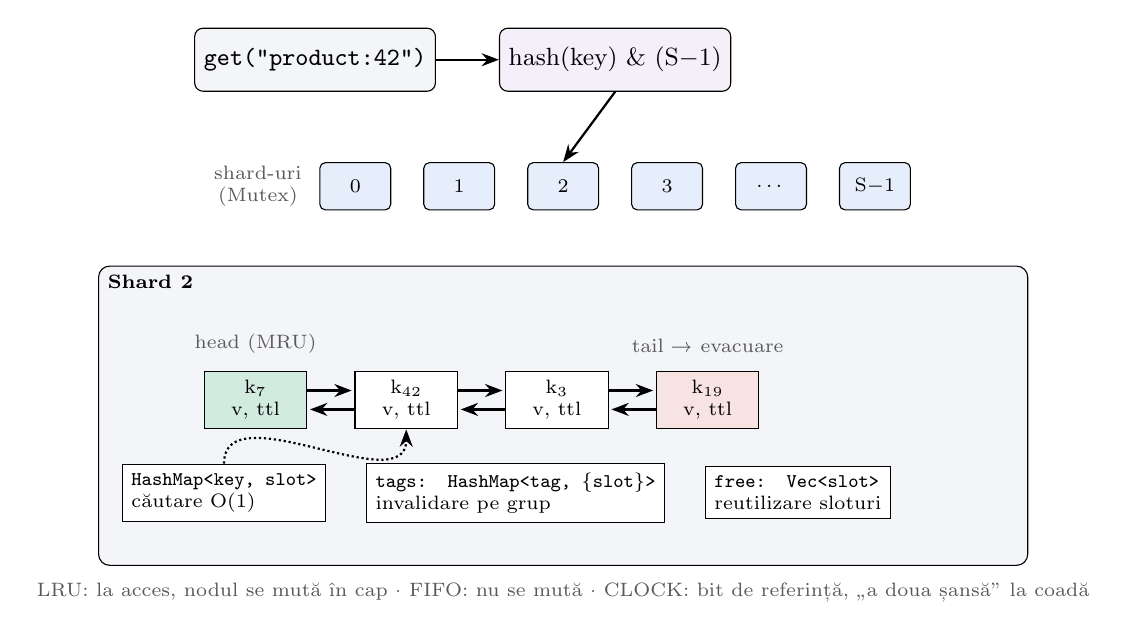
\begin{tikzpicture}[
  slot/.style={draw, minimum width=13mm, minimum height=7mm, font=\scriptsize, fill=white, align=center},
  sh/.style={draw, rounded corners=2pt, minimum width=9mm, minimum height=6mm, font=\scriptsize, fill=c1!12}]
  \node[comp, minimum width=26mm] (k) {\texttt{get("product:42")}};
  \node[comp, right=8mm of k, minimum width=24mm, fill=c4!10] (h) {hash(key) \& (S$-$1)};
  \draw[arr] (k) -- (h);
  \foreach \i in {0,...,5} { \node[sh] (s\i) at ($(h.south)+(-3.3+1.32*\i,-1.2)$) {\ifnum\i=5 S$-$1\else\ifnum\i=4 …\else\i\fi\fi}; }
  \draw[arr] (h.south) -- (s2.north);
  \node[note, left=1mm of s0] {shard-uri\\(Mutex)};

  % Detaliul unui shard.
  \node[draw, rounded corners, fill=boxbg, minimum width=118mm, minimum height=38mm, below=7mm of s2.south, anchor=north] (box) {};
  \node[font=\scriptsize\bfseries, anchor=north west] at (box.north west) {Shard 2};
  \node[slot, fill=c3!20] (e1) at ($(box.west)+(20mm,2mm)$) {k$_7$\\v, ttl};
  \node[slot, right=6mm of e1] (e2) {k$_{42}$\\v, ttl};
  \node[slot, right=6mm of e2] (e3) {k$_3$\\v, ttl};
  \node[slot, right=6mm of e3, fill=c5!15] (e4) {k$_{19}$\\v, ttl};
  \foreach \a/\b in {e1/e2,e2/e3,e3/e4} {
    \draw[arr, shorten >=1pt] ([yshift=1.2mm]\a.east) -- ([yshift=1.2mm]\b.west);
    \draw[arr, shorten >=1pt] ([yshift=-1.2mm]\b.west) -- ([yshift=-1.2mm]\a.east);
  }
  \node[note, above=1mm of e1] {head (MRU)};
  \node[note, above=1mm of e4] {tail → evacuare};
  \node[draw, font=\scriptsize, align=left, fill=white, anchor=north west] (map) at ($(box.south west)+(3mm,13mm)$) {\texttt{HashMap<key, slot>}\\ căutare O(1)};
  \node[draw, font=\scriptsize, align=left, fill=white, right=5mm of map] (tags) {\texttt{tags: HashMap<tag, \{slot\}>}\\ invalidare pe grup};
  \node[draw, font=\scriptsize, align=left, fill=white, right=5mm of tags] (free) {\texttt{free: Vec<slot>}\\ reutilizare sloturi};
  \draw[arr, densely dotted] (map.north) to[out=90,in=-90] (e2.south);
  \node[note, below=1mm of box] {LRU: la acces, nodul se mută în cap · FIFO: nu se mută · CLOCK: bit de referință, „a doua șansă" la coadă};
\end{tikzpicture}
}\\[2mm]
  \footnotesize Shard-uri cu mutex propriu · slab + listă intrusivă · O(1) · LRU/FIFO/CLOCK · TTL · tag-uri
\end{frame}

\begin{frame}{Cache distribuit și citirea cu single-flight}
  \begin{columns}[c]
    \column{0.33\textwidth}\centering
    \resizebox{\linewidth}{!}{% Inelul de consistent hashing cu noduri virtuale.
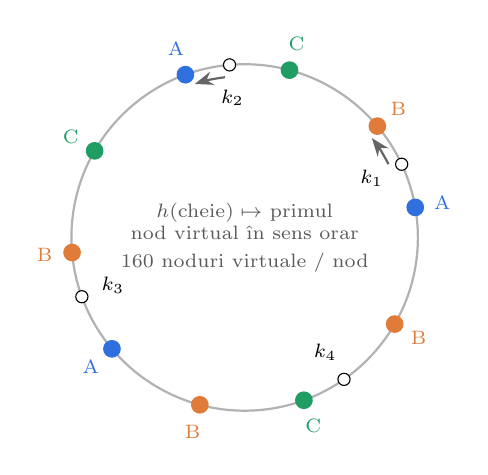
\begin{tikzpicture}
  \def\R{2.2}
  \draw[thick, gray!60] (0,0) circle (\R);
  \foreach \ang/\col/\lab in {10/c1/A,40/c2/B,75/c3/C,110/c1/A,150/c3/C,185/c2/B,220/c1/A,255/c2/B,290/c3/C,330/c2/B} {
    \fill[\col] (\ang:\R) circle (3.2pt);
    \node[font=\scriptsize, text=\col] at (\ang:\R+0.35) {\lab};
  }
  \foreach \ang/\k in {25/k_1,95/k_2,200/k_3,305/k_4} {
    \draw[fill=white, draw=black] (\ang:\R) circle (2.2pt);
    \node[font=\scriptsize] at (\ang:\R-0.42) {$\k$};
  }
  \draw[-{Stealth}, thick, black!60] (27:\R-0.15) arc (27:38:\R-0.15);
  \draw[-{Stealth}, thick, black!60] (97:\R-0.15) arc (97:108:\R-0.15);
  \node[note, align=center] at (0,0) {$h(\text{cheie}) \mapsto$ primul\\nod virtual în sens orar\\[2pt] 160 noduri virtuale / nod};
\end{tikzpicture}
}\\[2mm]
    \scriptsize consistent hashing, 160 noduri virtuale\\ protocol TCP propriu, pipelining
    \column{0.65\textwidth}\centering
    \resizebox{\linewidth}{!}{% Diagrama de secvență: citire cache-aside cu single-flight.
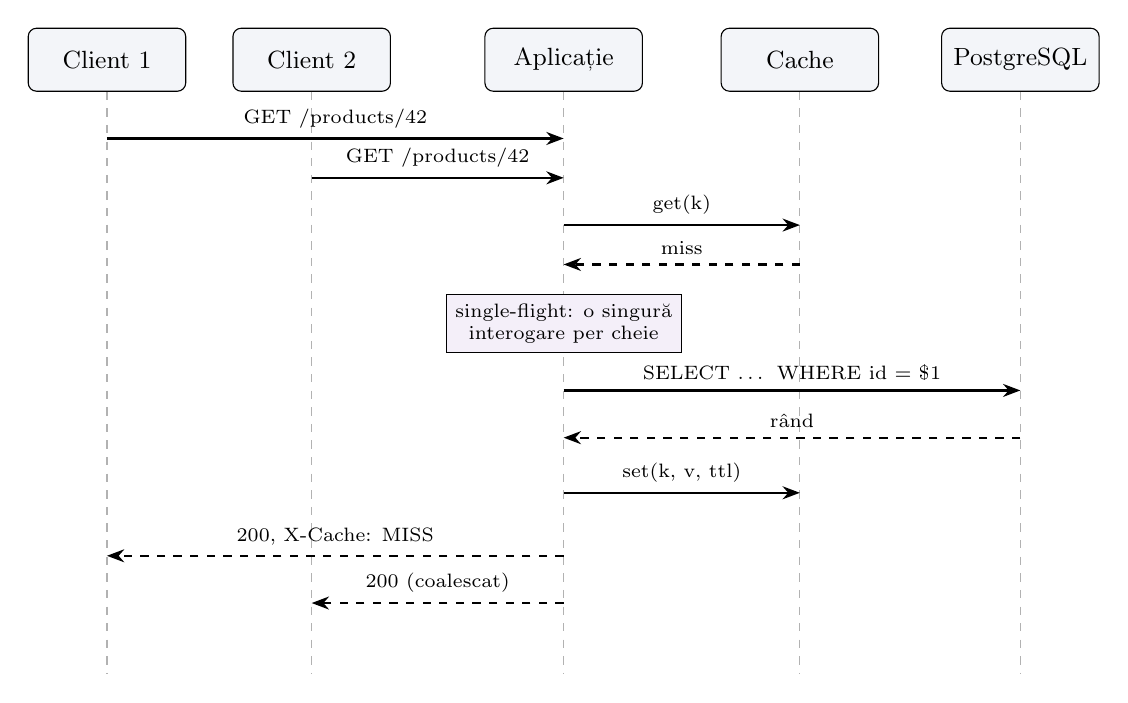
\begin{tikzpicture}[font=\small]
  \foreach \x/\n/\t in {0/c1/Client 1,2.6/c2/Client 2,5.8/app/Aplicație,8.8/cache/Cache,11.6/db/PostgreSQL} {
    \node[comp, minimum width=20mm] (\n) at (\x,0) {\t};
    \draw[gray!60, dashed] (\n.south) -- ++(0,-7.4);
  }
  \newcommand{\msg}[5][]{\draw[arr,#1] (#2,#4) -- node[above, font=\scriptsize]{#5} (#3,#4);}
  \msg{0}{5.8}{-1.0}{GET /products/42}
  \msg{2.6}{5.8}{-1.5}{GET /products/42}
  \msg{5.8}{8.8}{-2.1}{get(k)}
  \msg[dashed]{8.8}{5.8}{-2.6}{miss}
  \node[draw, fill=c4!10, font=\scriptsize, align=center] at (5.8,-3.35) {single-flight: o singură\\interogare per cheie};
  \msg{5.8}{11.6}{-4.2}{SELECT … WHERE id = \$1}
  \msg[dashed]{11.6}{5.8}{-4.8}{rând}
  \msg{5.8}{8.8}{-5.5}{set(k, v, ttl)}
  \msg[dashed]{5.8}{0}{-6.3}{200, X-Cache: MISS}
  \msg[dashed]{5.8}{2.6}{-6.9}{200 (coalescat)}
\end{tikzpicture}
}
  \end{columns}
\end{frame}

\begin{frame}{Strategii de scriere și coerență}
  \centering\resizebox{0.95\linewidth}{!}{% Cele trei strategii de scriere.
\begin{tikzpicture}[font=\small, node distance=4mm]
  \foreach \col/\x/\title/\a/\b/\c in {
      c1/0/Invalidate (cache-aside)/1. UPDATE în DB/2. DEL cheie din cache/3. următoarea citire: miss → DB,
      c3/5.2/Write-through/1. UPDATE în DB/2. SET valoarea nouă în cache/3. citirile rămân hit,
      c2/10.4/Write-behind/1. SET în cache; răspuns 202/2. coadă → lot (≤1024)/3. un UPDATE … unnest()} {
    \node[draw=\col, very thick, rounded corners, minimum width=48mm, minimum height=27mm, fill=\col!6] (b) at (\x,0) {};
    \node[font=\small\bfseries, text=\col, anchor=north] at (b.north) {\title};
    \node[font=\scriptsize, align=left, anchor=north west] at ($(b.north west)+(2mm,-7mm)$) {\a\\[2pt]\b\\[2pt]\c};
  }
  \node[note, text width=46mm] at (0,-2.0) {+ simplu, corect\\− miss după fiecare scriere};
  \node[note, text width=46mm] at (5.2,-2.0) {+ hit ratio păstrat\\− latență de scriere mai mare};
  \node[note, text width=46mm] at (10.4,-2.0) {+ scrieri rapide, grupate\\− consistență eventuală, risc la crash};
\end{tikzpicture}
}
  \vspace{3mm}
  \begin{itemize}\small
    \item Coerența L1 între instanțe: trigger PostgreSQL $\rightarrow$ \texttt{NOTIFY} $\rightarrow$ \texttt{LISTEN} în fiecare instanță
    \item Test end-to-end: \alert{18/18} combinații backend × strategie coerente
  \end{itemize}
\end{frame}

\begin{frame}{Șase backend-uri, comutabile la runtime}
  \small
  \begin{tabular}{ll}
    \toprule
    \texttt{none} & fără cache — baseline \\
    \texttt{local} & \texttt{memtable} în proces (L1) \\
    \texttt{cluster} & 3 noduri \texttt{cache-node}, consistent hashing \\
    \texttt{tiered} & L1 local (TTL 5 s) + L2 cluster — near-cache \\
    \texttt{redis} & Redis 8 — baseline industrial \\
    \texttt{pgmem} & tabelă \texttt{UNLOGGED} în PostgreSQL pe \texttt{tmpfs} — „tabelă in-memory" relațională \\
    \bottomrule
  \end{tabular}
  \vspace{4mm}

  UI de control · Swagger/OpenAPI · Prometheus + Grafana · Docker Compose (11 servicii)
\end{frame}

\begin{frame}{Optimizări ghidate de profilare}
  \small
  \begin{enumerate}
    \item Profilare: \alert{PostgreSQL la 410\% CPU}, aplicațiile sub 20\%
    \item Fără paralelism intra-query + indecși acoperitori $\Rightarrow$ clasament 7,6 ms $\rightarrow$ 1,5 ms
    \item Calea fierbinte: mimalloc, metrici pre-rezolvate, fără tracing per cerere
    \item \texttt{NOTIFY} serializa toate commit-urile (\texttt{Lock:object}) $\Rightarrow$ notificare doar când există L1
    \item Agregate materializate + index $\Rightarrow$ clasament \alert{0,09 ms}; PostgreSQL de la 410\% la $\approx$60–100\% CPU
  \end{enumerate}
  \vspace{2mm}
  \begin{center}
  \begin{tabular}{lrr}
    \toprule
    & înainte & după \\ \midrule
    fără cache (cereri/s) & \R{opt/baseline-none/rps} & \R{opt/mat-none/rps} \\
    cache local (cereri/s) & \R{opt/baseline/rps} & \R{opt/mat-local/rps} \\
    cache local p99 (ms) & \R{opt/baseline/p99} & \R{opt/mat-local/p99} \\
    \bottomrule
  \end{tabular}
  \end{center}
\end{frame}

\section{Rezultate experimentale}

\begin{frame}{Metodologie}
  \begin{itemize}
    \item 5 vCPU (Docker Desktop), toate componentele pe aceeași mașină
    \item \texttt{loadgen} propriu: closed-loop, Zipf, histograme HDR, 5 s încălzire + 15 s măsurare
    \item Implicit: 64 clienți, 95\% citiri (10\% dintre ele clasamente), Zipf $s=0{,}99$
    \item 8 experimente HTTP + 2 benchmark-uri offline; totul scriptat (\texttt{make bench})
  \end{itemize}
\end{frame}

\begin{frame}{E1 — comparația backend-urilor}
  \centering\resizebox{0.95\linewidth}{!}{% E1 — comparația backend-urilor.
\begin{tikzpicture}
\begin{groupplot}[group style={group size=2 by 1, horizontal sep=17mm},
    width=0.5\linewidth, height=55mm, ybar, xtick=data,
    symbolic x coords={none,local,cluster,tiered,redis,pgmem},
    x tick label style={rotate=35, anchor=east, font=\footnotesize}, enlarge x limits=0.1]
  \nextgroupplot[ylabel={cereri / s}, bar width=8pt, ymin=0,
      nodes near coords, nodes near coords style={font=\tiny, rotate=90, anchor=west},
      point meta={\thisrow{rps}/1000}, nodes near coords={\pgfmathprintnumber[fixed,precision=1]{\pgfplotspointmeta}k},
      kticks, ymax=88000,
      title={\small (a) debit}]
    \addplot[fill=c1!70, draw=c1] table[x=backend, y=rps, col sep=comma] {\datadir e1.csv};
  \nextgroupplot[ylabel={latență (ms)}, ymode=log, bar width=5pt, log origin=infty,
      legend style={at={(0.02,0.98)}, anchor=north west}, title={\small (b) latență}]
    \addplot[fill=c3!70, draw=c3] table[x=backend, y=p50, col sep=comma] {\datadir e1.csv};
    \addplot[fill=c2!70, draw=c2] table[x=backend, y=p95, col sep=comma] {\datadir e1.csv};
    \addplot[fill=c5!70, draw=c5] table[x=backend, y=p99, col sep=comma] {\datadir e1.csv};
    \legend{p50, p95, p99}
\end{groupplot}
\end{tikzpicture}
}
\end{frame}

\begin{frame}{E2 — asimetria Zipf (cache = 10\% din chei)}
  \centering\resizebox{0.95\linewidth}{!}{% E2 — asimetria Zipf (cache = 10% din chei, doar citiri).
\begin{tikzpicture}
\begin{groupplot}[group style={group size=2 by 1, horizontal sep=17mm},
    width=0.5\linewidth, height=55mm, xlabel={exponent Zipf $s$}, xtick={0.6,0.8,0.99,1.2}]
  \nextgroupplot[ylabel={rata de hit}, ymin=0, ymax=1, legend pos=south east, title={\small (a) rata de hit}]
    \addplot table[x=label, y=local_hit_ratio, col sep=comma] {\datadir e2.csv};
    \addplot table[x=label, y=cluster_hit_ratio, col sep=comma] {\datadir e2.csv};
    \addplot[c6, thick, dashed, mark=o] table[x=label, y=ideal, col sep=comma] {\datadir e2.csv};
    \legend{local, cluster, ideal IRM}
  \nextgroupplot[ylabel={cereri / s}, ymin=0, legend pos=north west, title={\small (b) debit},
      kticks]
    \addplot[c6, mark=o, thick] table[x=label, y=none_throughput_rps, col sep=comma] {\datadir e2.csv};
    \addplot table[x=label, y=local_throughput_rps, col sep=comma] {\datadir e2.csv};
    \addplot table[x=label, y=cluster_throughput_rps, col sep=comma] {\datadir e2.csv};
    \legend{none, local, cluster}
\end{groupplot}
\end{tikzpicture}
}
\end{frame}

\begin{frame}{E3 — strategii de scriere}
  \centering\resizebox{0.95\linewidth}{!}{% E3 — strategii de scriere.
\begin{tikzpicture}
\begin{groupplot}[group style={group size=2 by 1, horizontal sep=17mm},
    width=0.5\linewidth, height=55mm, xlabel={proporția de citiri}, xtick={0.5,0.8,0.95}]
  \nextgroupplot[ylabel={cereri / s}, ymin=0, legend pos=south east, title={\small (a) debit},
      kticks]
    \addplot table[x=label, y=invalidate_throughput_rps, col sep=comma] {\datadir e3.csv};
    \addplot table[x=label, y=write-through_throughput_rps, col sep=comma] {\datadir e3.csv};
    \addplot table[x=label, y=write-behind_throughput_rps, col sep=comma] {\datadir e3.csv};
    \legend{invalidate, write-through, write-behind}
  \nextgroupplot[ylabel={tranzacții DB / 1000 scrieri}, ymode=log, ymin=150, ymax=1300, ytick={200,300,500,1000}, log ticks with fixed point,
      title={\small (b) scrieri în DB}]
    \addplot table[x=label, y=invalidate_tx_per_1k, col sep=comma] {\datadir e3.csv};
    \addplot table[x=label, y=write-through_tx_per_1k, col sep=comma] {\datadir e3.csv};
    \addplot table[x=label, y=write-behind_tx_per_1k, col sep=comma] {\datadir e3.csv};
\end{groupplot}
\end{tikzpicture}
}
\end{frame}

\begin{frame}{E4 — scalabilitate cu numărul de clienți}
  \centering\resizebox{0.95\linewidth}{!}{% E4 — scalabilitatea cu numărul de clienți.
\begin{tikzpicture}
\begin{groupplot}[group style={group size=2 by 1, horizontal sep=17mm},
    width=0.5\linewidth, height=55mm, xlabel={clienți concurenți}, xmode=log, log basis x=2,
    xtick={1,4,16,64,256}, xticklabels={1,4,16,64,256}]
  \nextgroupplot[ylabel={cereri / s}, ymin=0, legend pos=north west, title={\small (a) debit},
      kticks]
    \addplot[c6, mark=o, thick] table[x=label, y=none_throughput_rps, col sep=comma] {\datadir e4.csv};
    \addplot table[x=label, y=local_throughput_rps, col sep=comma] {\datadir e4.csv};
    \addplot table[x=label, y=cluster_throughput_rps, col sep=comma] {\datadir e4.csv};
    \legend{none, local, cluster}
  \nextgroupplot[ylabel={latență p99 (ms)}, ymode=log, legend pos=north west, title={\small (b) latență p99}]
    \addplot[c6, mark=o, thick] table[x=label, y=none_p99_ms, col sep=comma] {\datadir e4.csv};
    \addplot table[x=label, y=local_p99_ms, col sep=comma] {\datadir e4.csv};
    \addplot table[x=label, y=cluster_p99_ms, col sep=comma] {\datadir e4.csv};
\end{groupplot}
\end{tikzpicture}
}
\end{frame}

\begin{frame}{E5–E7 — scale-out, memorie agregată, stampede}
  \centering\resizebox{0.98\linewidth}{!}{% E5 scale-out, E6 noduri, E7 stampede.
\begin{tikzpicture}
\begin{groupplot}[group style={group size=3 by 1, horizontal sep=21mm}, width=0.36\linewidth, height=52mm]
  \nextgroupplot[ybar, bar width=9pt, ymin=0, xtick={1,2}, xlabel={instanțe web}, ylabel={cereri / s},
      enlarge x limits=0.6, ymax=108000, legend columns=2, legend style={at={(0.5,0.98)}, anchor=north},
      kticks, title={\small (a) E5: scale-out}]
    \addplot[fill=c6!50, draw=c6] table[x=label, y=none_throughput_rps, col sep=comma] {\datadir e5.csv};
    \addplot[fill=c2!70, draw=c2] table[x=label, y=cluster_throughput_rps, col sep=comma] {\datadir e5.csv};
    \legend{none, cluster}
  \nextgroupplot[xtick={1,2,3}, xlabel={noduri de cache}, ylabel={rata de hit}, ymin=0, ymax=1,
      title={\small (b) E6: memorie agregată}]
    \addplot table[x=label, y=cluster_hit_ratio, col sep=comma] {\datadir e6.csv};
  \nextgroupplot[ybar, bar width=16pt, ymin=0, xtick={0,1}, xticklabels={fără, cu}, xlabel={single-flight},
      ylabel={interogări DB}, enlarge x limits=0.6, scaled y ticks=false, ymax=170000,
      yticklabel={\pgfmathprintnumber[fixed]{\tick}}, title={\small (c) E7: stampede}]
    \addplot[fill=c5!60, draw=c5] table[x=coalesce, y=db_reads, col sep=comma] {\datadir e7.csv};
\end{groupplot}
\end{tikzpicture}
}
\end{frame}

\begin{frame}{E8 — costul CPU la debit fix}
  \centering\resizebox{0.95\linewidth}{!}{% E8 — CPU consumat la debit fix (8.000 cereri/s), pe roluri.
\begin{tikzpicture}
\begin{axis}[width=0.8\linewidth, height=60mm, ybar stacked, bar width=14pt, ymin=0,
    symbolic x coords={none,local,cluster,tiered,redis,pgmem}, xtick=data,
    ylabel={CPU (\% dintr-un nucleu)}, legend style={at={(1.02,1)}, anchor=north west},
    enlarge x limits=0.12, reverse legend]
  \addplot[fill=c3!70, draw=c3] table[x=backend, y=app, col sep=comma] {\datadir e8.csv};
  \addplot[fill=c1!70, draw=c1] table[x=backend, y=db, col sep=comma] {\datadir e8.csv};
  \addplot[fill=c2!70, draw=c2] table[x=backend, y=cache, col sep=comma] {\datadir e8.csv};
  \addplot[fill=c6!35, draw=c6] table[x=backend, y=nginx, col sep=comma] {\datadir e8.csv};
  \legend{aplicație, PostgreSQL, servere de cache, nginx}
\end{axis}
\end{tikzpicture}
}
\end{frame}

\begin{frame}{Politici de evacuare (simulare)}
  \centering\resizebox{!}{0.85\textheight}{% Simulare politici de evacuare.
\begin{tikzpicture}
\begin{groupplot}[group style={group size=2 by 2, horizontal sep=17mm, vertical sep=18mm},
    width=0.5\linewidth, height=50mm, xmode=log, xtick={1,2,5,10,20,50}, xticklabels={1,2,5,10,20,50},
    xlabel={capacitate (\% din chei)}, ylabel={rata de hit}, ymin=0, ymax=1]
  \nextgroupplot[title={\small Zipf $s=0{,}8$}, legend pos=north west]
    \addplot table[x=cap, y=lru, col sep=comma] {\datadir sim_zipf_08.csv};
    \addplot table[x=cap, y=fifo, col sep=comma] {\datadir sim_zipf_08.csv};
    \addplot table[x=cap, y=clock, col sep=comma] {\datadir sim_zipf_08.csv};
    \addplot[c6, thick, dashed] table[x=cap, y=ideal, col sep=comma] {\datadir sim_zipf_08.csv};
    \legend{LRU, FIFO, CLOCK, ideal}
  \nextgroupplot[title={\small Zipf $s=0{,}99$}]
    \addplot table[x=cap, y=lru, col sep=comma] {\datadir sim_zipf_099.csv};
    \addplot table[x=cap, y=fifo, col sep=comma] {\datadir sim_zipf_099.csv};
    \addplot table[x=cap, y=clock, col sep=comma] {\datadir sim_zipf_099.csv};
    \addplot[c6, thick, dashed] table[x=cap, y=ideal, col sep=comma] {\datadir sim_zipf_099.csv};
  \nextgroupplot[title={\small Zipf $s=0{,}8$ + 20\% scanări}]
    \addplot table[x=cap, y=lru, col sep=comma] {\datadir sim_zipf_scan_08.csv};
    \addplot table[x=cap, y=fifo, col sep=comma] {\datadir sim_zipf_scan_08.csv};
    \addplot table[x=cap, y=clock, col sep=comma] {\datadir sim_zipf_scan_08.csv};
  \nextgroupplot[title={\small Zipf $s=0{,}99$ + 20\% scanări}]
    \addplot table[x=cap, y=lru, col sep=comma] {\datadir sim_zipf_scan_099.csv};
    \addplot table[x=cap, y=fifo, col sep=comma] {\datadir sim_zipf_scan_099.csv};
    \addplot table[x=cap, y=clock, col sep=comma] {\datadir sim_zipf_scan_099.csv};
\end{groupplot}
\end{tikzpicture}
}
\end{frame}

\begin{frame}{Scalabilitatea motorului: fire × shard-uri}
  \centering\resizebox{0.95\linewidth}{!}{% Scalabilitatea motorului memtable.
\begin{tikzpicture}
\begin{groupplot}[group style={group size=2 by 1, horizontal sep=17mm},
    width=0.5\linewidth, height=58mm, xlabel={fire}, xtick={1,2,4,5,8}]
  \nextgroupplot[ylabel={Mops / s}, ymin=0, ymax=19, title={\small (a) debit (LRU, Zipf 0{,}99)},
      legend style={font=\scriptsize, at={(0.02,0.98)}, anchor=north west}, legend columns=2]
    \addplot table[x=threads, y=s1_mops, col sep=comma] {\datadir engine.csv};
    \addplot table[x=threads, y=s4_mops, col sep=comma] {\datadir engine.csv};
    \addplot table[x=threads, y=s16_mops, col sep=comma] {\datadir engine.csv};
    \addplot table[x=threads, y=s64_mops, col sep=comma] {\datadir engine.csv};
    \legend{1 shard, 4 shard-uri, 16 shard-uri, 64 shard-uri}
  \nextgroupplot[ylabel={accelerare $S(p)$}, ymin=0, ymax=8, title={\small (b) accelerare, 64 shard-uri},
      legend style={font=\scriptsize, at={(0.02,0.98)}, anchor=north west}]
    \addplot table[x=threads, y=s64_speedup, col sep=comma] {\datadir engine.csv};
    \addplot table[x=threads, y=s64clock_speedup, col sep=comma] {\datadir engine.csv};
    \addplot table[x=threads, y=s64unif_speedup, col sep=comma] {\datadir engine.csv};
    \addplot[c5, mark=pentagon*, thick] table[x=threads, y=s1_speedup, col sep=comma] {\datadir engine.csv};
    \addplot[c6, dashed, thick, domain=1:8, samples=9, mark=none] {min(x,5)};
    \legend{{LRU, Zipf 0{,}99}, {CLOCK, Zipf 0{,}99}, LRU uniform, 1 shard (LRU), ideal}
\end{groupplot}
\end{tikzpicture}
}
\end{frame}

\begin{frame}{Concluzii}
  \small
\begin{itemize}
  \item \alert{Întâi baza de date, apoi cache-ul}: \R{opt/baseline/rps} $\rightarrow$ \R{opt/mat-local/rps} cereri/s, p99 \R{opt/baseline/p99} $\rightarrow$ \R{opt/mat-local/p99} ms
  \item Cache local: \R{e1/local/speedup}× debit față de DB optimizat, $-$27\% CPU per cerere
  \item Cache partajat (cluster, Redis): hit mai mare, coerență mai ieftină; prag de rentabilitate (E2)
  \item Tabela in-memory în SGBD (\texttt{pgmem}): \alert{mai lentă decât DB-ul} pentru date deja în RAM
  \item Write-behind: debit maxim, de câteva ori mai puține tranzacții, consistență eventuală
  \item Sharding: de la colaps (1 shard) la scalare; cheile fierbinți limitează accelerarea
  \item Single-flight: $-$29\% interogări la pornirea la rece; coerență 18/18
\end{itemize}

\end{frame}

\begin{frame}[standout]
  Întrebări?\\[4mm]
  \normalsize\texttt{make up} $\rightarrow$ \texttt{http://localhost:8080}
\end{frame}

\end{document}
